\maketitle
\chapter{FSM ed AXI-Stream}
\section{Implementazione della FSM e Interfacce AXI-Stream}

Il cuore del sistema di filtraggio è costituito dalla logica di controllo, implementata attraverso una Macchina a Stati Finiti (FSM) che orchestra il riempimento dei \textit{buffer line}, la generazione della finestra $3 \times 3$ e la gestione dei segnali del protocollo AXI4-Stream.
In questo capitolo vengono analizzati nel dettaglio il diagramma degli stati, la gestione dei segnali di sincronizzazione (SOF ed EOL) e la logica di controllo del flusso dati (\textit{backpressure}).

\subsection{Architettura della FSM}
La FSM ha il compito di coordinare tre segnali di controllo fondamentali per il funzionamento della pipeline:
\begin{itemize}
	\item \texttt{pipeline\_en}: segnale di abilitazione globale che determina l'avanzamento dei dati nei registri a scorrimento;
	\item \texttt{window\_valid}: flag che indica se la finestra di convoluzione attuale contiene dati validi per il calcolo;
	\item \texttt{flush\_pipeline}: segnale che gestisce la fase terminale dell'elaborazione, forzando l'ingresso a zero quando non vi sono più pixel in arrivo ma la pipeline deve ancora svuotarsi.
\end{itemize}

A differenza di implementazioni classiche, lo stato di \texttt{IDLE} è stato rimosso dalla logica esplicita degli stati per ottimizzare la risposta al segnale di \textit{Start Of Frame} (SOF). La macchina opera principalmente su tre stati:

\begin{enumerate}
	\item \textbf{LOADING}: In questa fase iniziale, il sistema riceve i dati in ingresso e riempie i \textit{line buffer}. La finestra di convoluzione non è ancora valida e l'uscita è disabilitata.
	\item \textbf{RUNNING}: Una volta riempita la finestra, il sistema entra in regime di elaborazione continua. Per ogni colpo di clock (se abilitato), viene prodotto un pixel filtrato in uscita.
	\item \textbf{FLUSH}: Alla ricezione dell'ultimo pixel dell'immagine, la macchina entra in fase di svuotamento. L'ingresso della pipeline viene alimentato con valori nulli (zero padding) per permettere l'elaborazione dei pixel ai bordi finali dell'immagine. Completato lo svuotamento, la FSM torna in attesa.
\end{enumerate}

\subsection{Gestione del Protocollo AXI4-Stream}
Il modulo agisce come un nodo di elaborazione trasparente all'interno della catena video, comportandosi come \textit{Slave} sull'interfaccia di ingresso e come \textit{Master} su quella di uscita.

\subsubsection{Interfaccia Slave (Ingresso)}
L'accettazione dei dati è governata dal segnale \texttt{s\_axis\_tready}. Questo viene asserito alto, segnalando la disponibilità a ricevere dati, a condizione che la FSM non si trovi nello stato di \texttt{FLUSH} e che il modulo a valle non stia esercitando \textit{backpressure}, ovvero la porta in uscita non è pronta a ricevere dati.
I segnali di controllo del frame vengono gestiti come segue:
\begin{itemize}
	\item \textbf{SOF (Start Of Frame - \texttt{tuser}):} Viene campionato per resettare istantaneamente la FSM e i contatori interni, garantendo l'allineamento all'inizio di ogni nuova immagine.
	\item \textbf{EOL (End Of Line - \texttt{tlast}):} Utilizzato per il conteggio delle righe e per innescare la transizione verso lo stato di \texttt{FLUSH} al termine del caricamento dell'ultimo pixel.
\end{itemize}

\subsubsection{Interfaccia Master (Uscita)}
In uscita, il segnale di validità \texttt{m\_axis\_tvalid} riflette lo stato interno del segnale \texttt{window\_valid}.
\begin{itemize}
	\item Il segnale \texttt{m\_axis\_tuser} viene asserito per un singolo ciclo di clock in corrispondenza del primo pixel valido uscente.
	\item Il segnale \texttt{m\_axis\_tlast} viene generato internamente da un contatore di colonne che traccia la posizione del pixel corrente all'interno della riga elaborata.
\end{itemize}

\subsection{Sincronizzazione e Rimozione dello stato IDLE}
Per massimizzare l'efficienza e la reattività, la logica di reset e avvio è basata sul segnale \texttt{s\_axis\_tuser}. Invece di attendere in uno stato inattivo, la FSM monitora costantemente l'arrivo di un nuovo frame.
Come mostrato nel Listing \ref{lst:sof_logic}, l'arrivo di un \texttt{tuser} alto forza la macchina nello stato di \texttt{LOADING} e azzera i contatori di latenza, indipendentemente dallo stato attuale.

\begin{lstlisting}[language=VHDL, caption={Gestione sincrona del SOF e reset implicito}, label={lst:sof_logic}]
	-- Processo Sincrono della FSM
	if rising_edge(s_axis_clk) then
		if s_axis_rstn = '0' then
			current_state <= LOADING;
	
	elsif pipeline_en_s = '1' then
		-- LOGICA DI SINCRONIZZAZIONE SOF
		-- Un TUSER valido indica SEMPRE l'inizio di un nuovo frame
		if s_axis_tvalid = '1' and s_axis_tuser = '1' then
			current_state    <= LOADING;
			latency_counter  <= 1;   -- Inizializzazione contatore
			flush_pipeline_s <= '0'; -- Interruzione flush precedenti
			m_axis_tuser_s   <= '0';
	else
		-- Evoluzione normale degli stati (LOADING, RUNNING, FLUSH)
	-- ...
	end if;
	end if;
	end if;
\end{lstlisting}

\subsection{Controllo del Dataflow e Backpressure}
La robustezza del filtro digitale in un contesto AXI-Stream dipende dalla corretta gestione della \textit{backpressure}. Il sistema deve essere in grado di "congelare" l'intera pipeline se il ricevitore a valle non è pronto ad accettare dati (\texttt{m\_axis\_tready = '0'}).

La logica combinatoria che genera il segnale di abilitazione \texttt{pipeline\_en\_s} è descritta dalla seguente espressione VHDL:

\begin{lstlisting}[language=VHDL, caption={Logica di abilitazione pipeline e gestione backpressure}, label={lst:pipeline_en}]
	pipeline_en_s <= '1' when ((s_axis_tvalid = '1' or current_state = FLUSH)
			and (m_axis_tready = '1' or window_valid_s = '0'))
			else '0';
	
	s_axis_tready <= '1' when (current_state /= FLUSH and m_axis_tready = '1') 
			else '0';
\end{lstlisting}

Analizzando il codice nel Listing \ref{lst:pipeline_en}, l'abilitazione avviene solo se:
\begin{enumerate}
	\item Vi è un dato valido in ingresso o la macchina è in fase di svuotamento (sorgente dati interna);
	\item \textbf{E} il ricevitore è pronto (\texttt{m\_axis\_tready = '1'}) o l'uscita attuale non è valida (quindi non c'è rischio di perdere dati).
\end{enumerate}

Se \texttt{m\_axis\_tready} scende a livello logico basso mentre è presente un dato valido in uscita, il segnale \texttt{pipeline\_en\_s} viene deasserito. Questo causa l'arresto immediato di tutti i registri a scorrimento e dei buffer, preservando lo stato interno del filtro fino a quando la congestione a valle non viene risolta.

\section{Verifica Funzionale: Integrazione FSM e Buffer Line}

Al fine di validare l'interazione tra la logica di controllo (FSM) e la pipeline di memoria (\textit{Buffer Line}), è stata sviluppata una testbench specifica. L'obiettivo principale è verificare la correttezza del protocollo AXI-Stream (gestione dell'handshake) e la coerenza dei dati in uscita durante le fasi critiche di \textit{Start of Frame} e \textit{Flush}.

\subsection{Setup di Simulazione}
Per facilitare l'analisi visiva delle waveform e il debug, i parametri del design sono stati ridotti rispetto alla configurazione di sintesi finale. Il setup di simulazione prevede:

\begin{itemize}
	\item \textbf{Dimensione Immagine:} Ridotta a $5 \times 5$ pixel (rispetto ai $32 \times 32$ o superiori del target reale). Questo permette di osservare un intero frame in un intervallo di tempo limitato.
	\item \textbf{Pattern Dati:} Generazione di un gradiente incrementale prevedibile. Il valore del pixel è calcolato come:
	\[
	P(row, col) = (row \times N_{col}) + col
	\]
	In questo modo, la sequenza di ingresso è composta da valori progressivi (0, 1, 2, \dots, 24), rendendo immediata l'identificazione di eventuali disallineamenti o perdite di dati nella pipeline.
	\item \textbf{Obiettivo:} La simulazione si concentra sui casi limite (corner cases): l'allineamento iniziale, la gestione della backpressure e il riempimento automatico (padding) durante la fase finale di flush.
\end{itemize}

\begin{figure}[htbp]
	\centering
	% Assicurati che il percorso dell'immagine sia corretto
	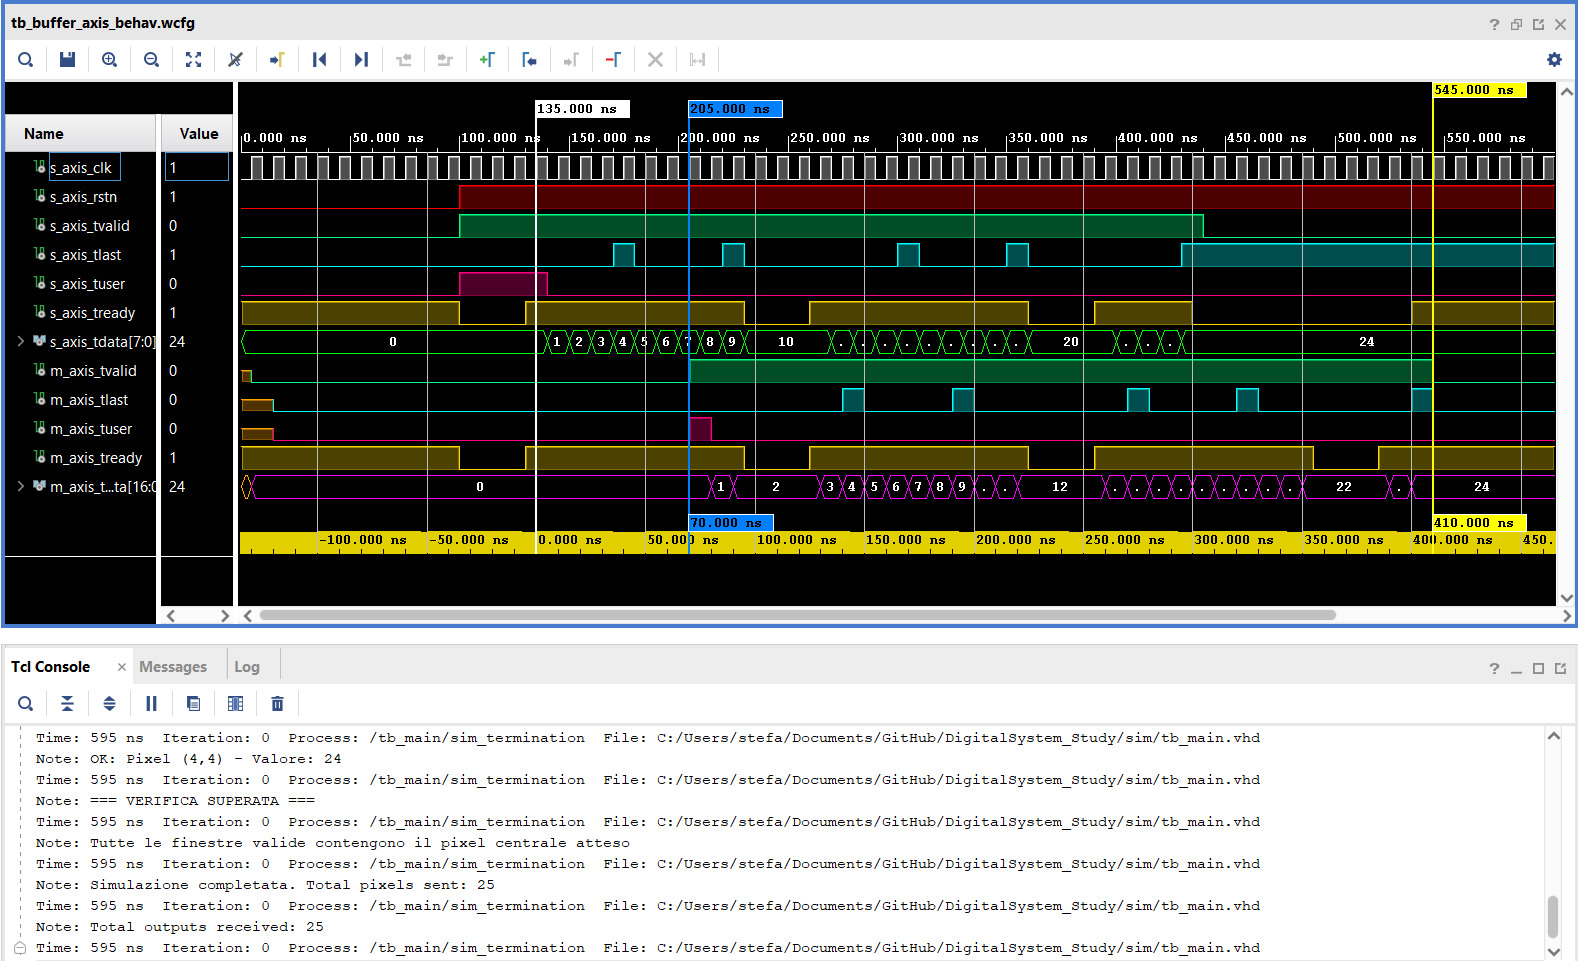
\includegraphics[width=\textwidth]{file_relazione/imgs/TB_waveforme_BL+FSM.png}
	\caption{Waveform della simulazione: interazione tra FSM e Buffer Line durante la fase di Flush.}
	\label{fig:tb_waveform}
\end{figure}

\subsection{Generazione degli Stimoli e Handshake AXI}
Il processo di stimolo della testbench emula una sorgente AXI-Stream Master. Un aspetto cruciale della verifica è la simulazione della \textit{backpressure}: il testbench non si limita a inviare dati, ma rispetta rigorosamente i segnali di controllo provenienti dal DUT (Device Under Test).

Nel Listing \ref{lst:tb_process} è riportato lo snippet VHDL che gestisce la generazione del frame. È fondamentale notare il loop di attesa su \texttt{s\_axis\_tready}: se la FSM abbassa il segnale di pronto (ad esempio durante un reset o una stallo interno), il generatore di stimoli sospende l'invio, garantendo la conformità al protocollo.

\begin{lstlisting}[language=VHDL, caption={Processo di generazione stimoli con gestione Handshake AXI}, label={lst:tb_process}]
	-- Processo di Stimolo: Generazione Immagine 5x5
	process
	begin
	-- Attesa reset...
	wait until rising_edge(clk);
	
	for row in 0 to NROW-1 loop
	for col in 0 to NCOL-1 loop
	-- Generazione Dato: Indice univoco per tracciabilita'
	s_axis_tdata  <= std_logic_vector(to_unsigned(row * NCOL + col, 8));
	s_axis_tvalid <= '1';
	
	-- Gestione Handshake (Backpressure Compliance)
	-- Il dato rimane valido finche' la FSM non e' pronta (tready = '1')
	loop
	wait until rising_edge(clk);
	exit when s_axis_tready = '1';
	end loop;
	
	end loop;
	end loop;
	
	-- Fine Frame: Disabilitazione validita' e attesa completamento flush
	s_axis_tvalid <= '0';
	wait for 100 ns;
	-- ...
	end process;
\end{lstlisting}

\subsection{Esiti della Verifica}
La simulazione ha confermato i seguenti comportamenti chiave:
\begin{enumerate}
	\item \textbf{Robustezza all'Handshake:} Il sistema gestisce correttamente le pause nel flusso dati. Quando \texttt{s\_axis\_tvalid} viene deasserito o quando la FSM deasserisce \texttt{s\_axis\_tready}, nessun dato viene perso o duplicato.
	\item \textbf{Automatismo del Flush:} Al termine dei loop di generazione (quando l'ultimo pixel valido entra nel sistema), la FSM rileva correttamente la condizione di fine frame. Come visibile in Figura \ref{fig:tb_waveform}, il segnale \texttt{flush\_pipeline} viene attivato internamente, forzando l'ingresso dei buffer a zero (padding). Questo permette alla finestra $3 \times 3$ di scorrere correttamente fino all'ultimo pixel dell'immagine, garantendo che l'output abbia le stesse dimensioni dell'input.
\end{enumerate}